%!TEX root = ../../main.tex

\chapter{Grundgerüst}
Im folgenden Abschnitten wird darauf eingegangen, welche Entwicklungsumgebung verwendet und eine virtuelle Umgebung in aufgesetzt wird. Darauf
wird die Versionsverwaltung mit Git erklärt und wie diese in PyCharm integriert ist. Der Abschluss dieses Kapitel
betrachtet die Ordnerstruktur des Code-Projektes.

\section{Einrichtung der Entwicklungsumgebung}
Als \acf{IDE} wird PyCharm von JetBrains verwendet. PyCharm bietet viele Möglichkeiten, um die Entwicklung
von Python-Programmen zu vereinfachen. Dazu gehören Debugging-Werkzeuge, Code-Vervollständigung, die Integration von Versionskontrolle
und die Option des Refactoring (\cite{pyCharmGettingStarted}).

\section{Einrichtung einer virtuellen Umgebung}
\glqq Eine virtuelle Umgebung oder Virtualenv Python Version ermöglicht es, mehrere parallele Instanzen
 des Python-Interpreters zu starten. Jede dieser Instanzen hat ihren 
 eigenen Satz an Paketen und ihre eigenen Konfigurationen. 
 Jede virtuelle Umgebung enthält auch eine Kopie des Python-Interpreters.\grqq (\cite{team_virtualenv_2023}).

 Die einzelnen Instanzen sind von einander isoliert. Wenn die Pakete in der einen virtuellen Umgebung angepasst werden, bleibt die andere Umgebung unverändert (\cite[S. 474]{hunt_beginners_2023}).

 In PyCharm ist sehr einfach eine neue virtuelle Umgebung anzulegen. Bei der Erstellung eines neuen Projektes, 
 lässt sich automatisch eine neue Umgebung hinzufügen. Hier ist es auch möglich, bereits vorhandene Umgebungen auszuwählen (vgl. \autoref{pyCharmVenv}).

 Es ist auch möglich, eine virtuelle Umgebung mit Interpreter nachzurüsten, wenn es bei der Projektezeugung vergessen worden ist.
 Dazu muss die Einstellung des Projektes unter dem Reiter \textit{Python Interpreter} ausgewählt werden (\cite{pyCharmVirtualEnv}).

 \begin{figure}[h]
    \centering
    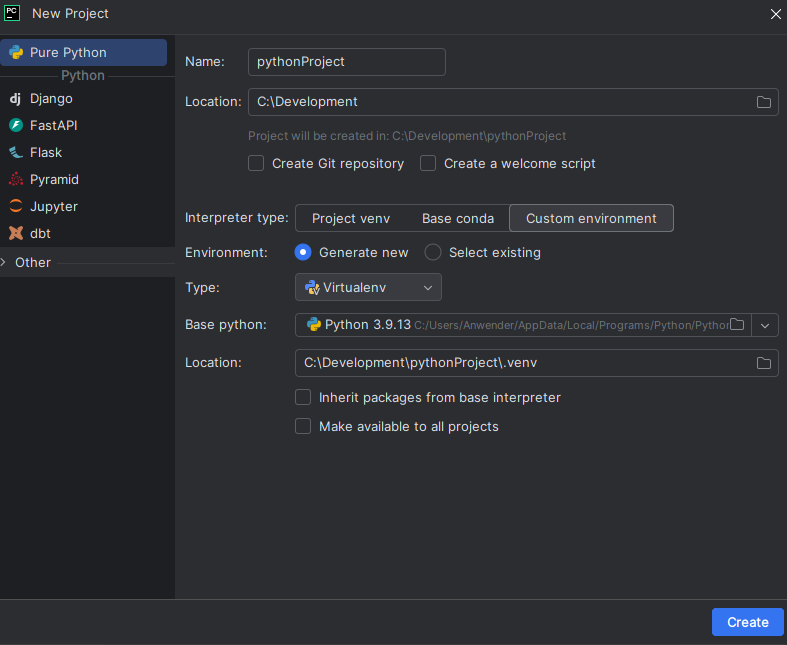
\includegraphics[height=.4\textwidth]{pycharm-Virtual-environment.png}
    \caption{Erstellung einer virtellen Umgebung in PyCharm}
    \label{pyCharmVenv}
    \end{figure}
\newpage
\section{Git-Integration}
Wenn viele Entwickler an dem gleichen Projekt arbeiten, kann es mal passieren, 
dass Fehler auftreten und der Code nicht mehr funktionsfähig ist. 
Aus diesem Grund ist es essenziel, ein Back-Up System zu haben, 
welche ältere, lauffähige Versionen wieder herstellen kann. 
Solche Systeme werden im allgemeinen als \acf{VCS} genannt. 
Ein sehr starkes, flexibles Tool, welches sehr gut für die Entwicklung in Teams geeignet ist, ist Git (\cite[S. 1]{loeliger_version_2012}).

Wie die virtuelle Umgebung, ist die Git-Integration in PyCharm sehr einfach gehalten.
In GitHub ist zunächst ein leeres Repository für das Projekt angelegt worden. Dieses Repository
wird in PyCharm geclonet (\cite{pyCharmGit}). Diesem Repository wird dann ein neues Python-Projekt mit virtueller Umgebung hinzugefügt (vgl. \autoref{pyCharmGit}).

\begin{figure}[h]
    \centering
    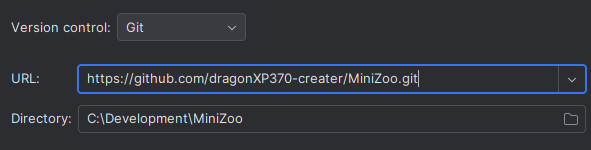
\includegraphics[]{pycharm-Git.png}
    \caption{Clone eines Git-Repository in PyCharm}
    \label{pyCharmGit}
\end{figure}

Alle Funktionen von Git, wie das Commiten von Änderungen oder das Management der unterschiedlichen Branches
lässt sich in der graphischen Oberfläche von PyCharm erledigen (vgl. \autoref{pyCharmGitCommit}).

\begin{figure}[h]
    \centering
    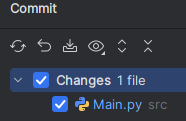
\includegraphics[]{pycharm-git-commit.png}
    \caption{Git-Commit in PyCharm}
    \label{pyCharmGitCommit}
\end{figure}

Ein wichtiger Bestandteil eines jeden Repositories ist die \textit{.gitignore}-Datei. 
Dadurch wird Git mitgeteilt, welche Dateien und Verzeichnise ignoriert werden müssen, damit diese nicht commited werden.
Mit dieser Datei lassen sich beispielsweise Einstellungen der verschiedenen \acp{IDE} ignorieren (\cite{github_Ignore}).

Über die Website \href{https://www.toptal.com/developers/gitignore/}{gitignore.io} lässt sich automatisch eine \textit{.gitignore}-Datei für alle gänigen \acp{IDE} erstellen (\cite{gitignore_io}).
Für dieses Projekt sind die Optionen \textit{PyCharm}, \textit{VisualStudio}, \textit{VisualStudioCode}, \textit{JetBrains+all} und \textit{Python} ausgewählt worden.

Das gesamte Projekt ist unter diesem Link verfügbar: \url{https://github.com/dragonXP370-creater/MiniZoo}

\section{Ordnerstruktur}
Das Projekt besteht aus drei Grundordnern. Der Ordner \textit{.venv} beinhaltet die virtuelle Umgebung und wird nicht weiter verändert.
Der Code des Programms ist in den Ordner \textit{src} und \textit{tests} aufgeteilt. Neben dem Main-Programm, beinhaltet der der \textit{src}-Ordner die Log-Datei
und die Unterordner \textit{Animals} und \textit{Exceptions}. Diese dienen dazu, um die Basisklasse und die verschiedenen Subklassen, bzw. die benutzerdefinierte Fehlermeldung, aufzubewahren.
Die Unit-Tests liegen in dem \textit{tests}-Verzeichznis ab (vgl. \autoref{folderStructure}).
\begin{figure}[h]
    \centering
    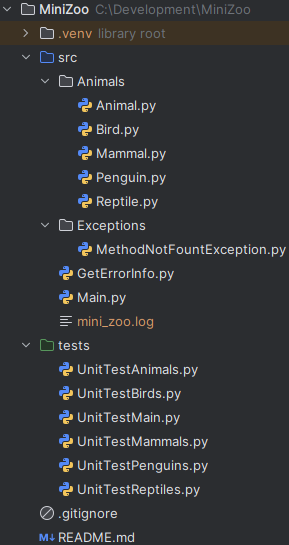
\includegraphics[height=10cm]{Ordner-Struktur.png}
    \caption{Ordnerstruktur}
    \label{folderStructure}
\end{figure}